%%%%%%%%%%%%%%%%%%%%%%%%%%%%%%%%%%%%%%%%%%%%%%%%%%%%%%%%%%%%%%%%%%%%%%%%
%                                                                      %
%     File: Thesis_Implementation.tex                                  %
%     Tex Master: Thesis.tex                                           %
%                                                                      %
%     Author: Andre C. Marta                                           %
%     Last modified :  2 Jul 2015                                      %
%                                                                      %
%%%%%%%%%%%%%%%%%%%%%%%%%%%%%%%%%%%%%%%%%%%%%%%%%%%%%%%%%%%%%%%%%%%%%%%%

\chapter{Proposal}
\label{chapter:implementation}


\begin{figure}[!htb]
  \centering
  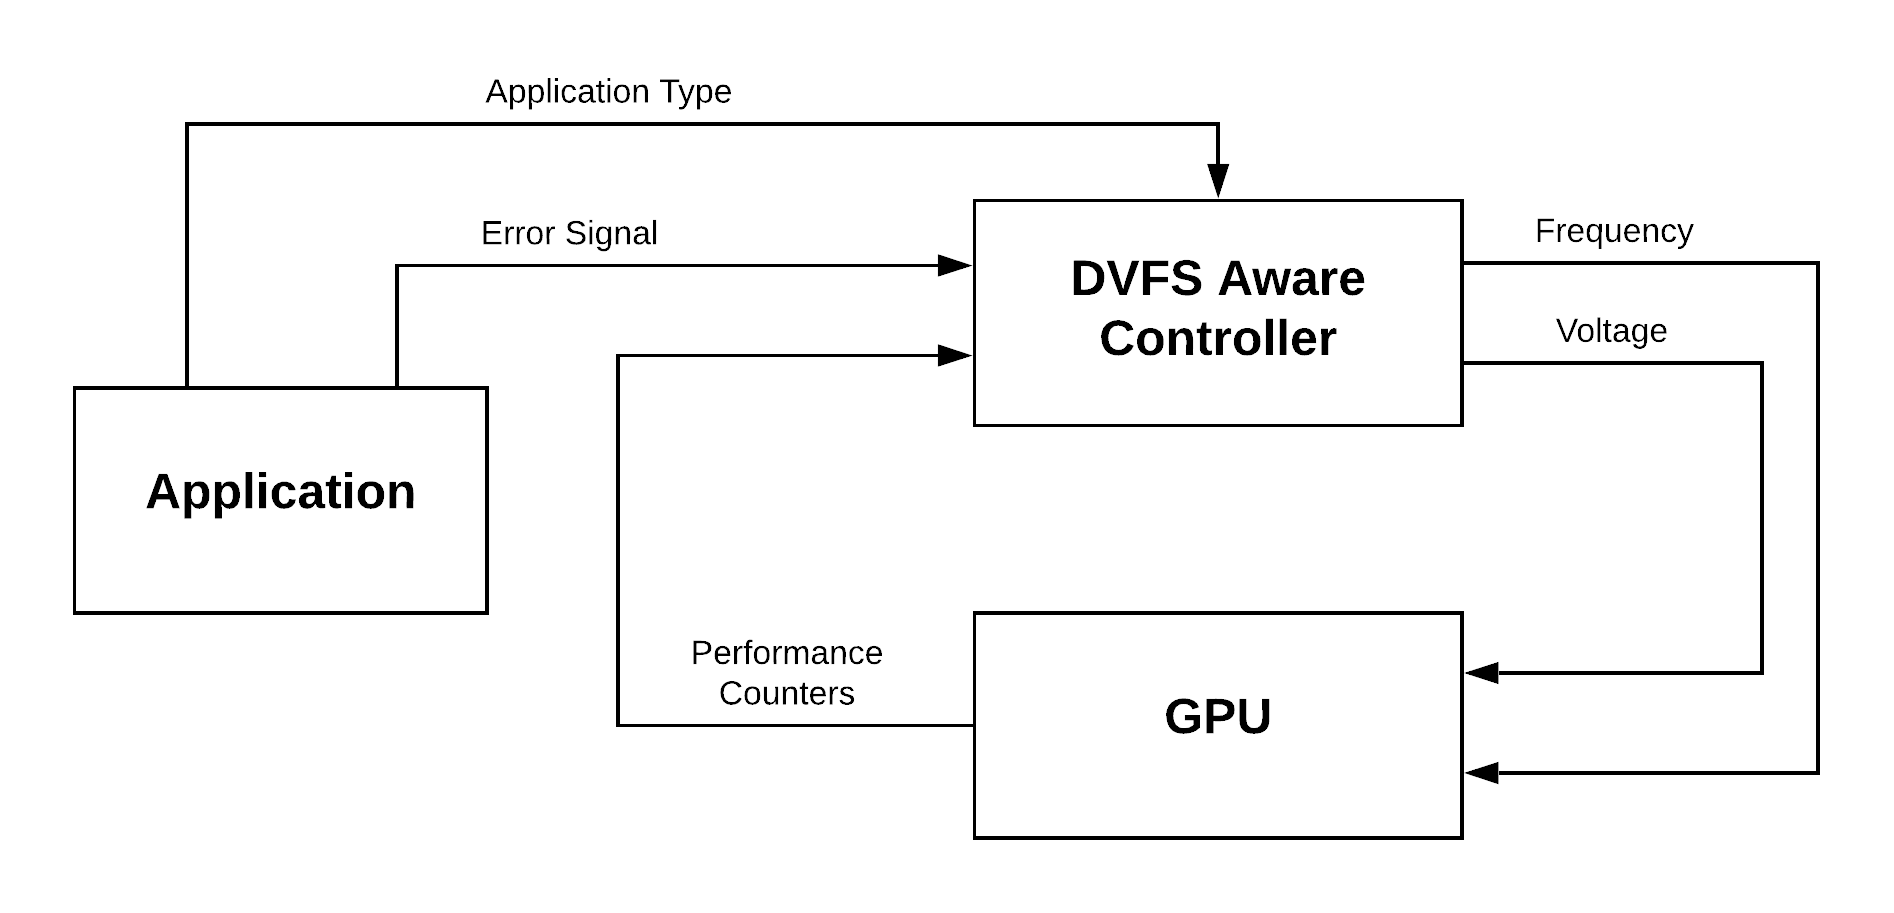
\includegraphics[width=0.75\textwidth]{Figures/Proposel/Controller_Diagram.png}
  \caption[Controller]{DVFS Aware Controller Block Diagram.}
  \label{fig:controlerDVFSaware}
\end{figure}



%%%%%%%%%%%%%%%%%%%%%%%%%%%%%%%%%%%%%%%%%%%%%%%%%%%%%%%%%%%%%%%%%%%%%%%%
\section{GPU DVFS Aware Mechanism}
\label{section:solarch}


%%%%%%%%%%%%%%%%%%%%%%%%%%%%%%%%%%%%%%%%%%%%%%%%%%%%%%%%%%%%%%%%%%%%%%%%
\subsection{Architecture of the Solution}
\label{section:solarch}

\subsection{Performance Counters}
\label{section:solarch}

\subsection{Neural Networks}
\label{section:solarch}

\section{Experimental Methodology}

To design the controller, it is necessary to first identify a set of artificial neural network models that are imprecision tolerant. Then, acquire meaningful metrics about the state of the GPU core and the quality of the output that the neural networks are producing. The second step is to study the relation between 

Analisar o comportamento da arquitetura da GPU à mudança de DVFS

Entender o comportamento da aprendisagem de modelos de machine learning - redes neuronais em particular - aquando da variação do ponto de funcionamento da GPU

Arranjar uma metodologia de analise da qualidade do output da aplicação e do estado do GPU

De modo a desenhar um controlador de tensao e frequencia realimentado 